\section{Results}
\label{sec:results}

We report three kinds of evidence, in decreasing order of completeness:
\begin{itemize}
\item functional bit-exactness of the whole recognizer;
\item a separately routed projection engine with scoped physical checks;
\item synthesizability of the whole recognizer for both silicon and FPGA.
\end{itemize}
The review reconciles the paper with archived reports and tool metrics; it does not rerun the silicon flow. Source files and their scopes are listed in \cref{app:artifacts}.

\subsection{Bit-exact recognition from index and codebook weights}
The full recognizer RTL decodes the clip ``Switch on the lights'' to the token sequence $[28176, 373, 278, 26068, 2]$. Eligible services use 4-bit indices into local 16-entry books; the frontend retains affine INT8 weights and supporting tables remain unchanged. All 18 checked output hashes match the reference, and the run takes \num{312578649} clocks, identical to the earlier byte-ROM design. Two further clips (``Plant present.'' and ``Seasonable.'') also match on all 18 hashes.

\Cref{tab:storage} covers the seven services converted in W11. Their storage falls from \SI{28.64}{MB} to \SI{17.50}{MB} ($-38.9\%$); decoding reproduces all \num{28641280} bytes of the frozen K64 byte-ROM baseline, not the original source model. Five unchanged tables add \num{8847360} bytes, giving \num{26344960} accounted bytes. Small LUTs and mutable state are excluded. The separate full-model software export and its 31.46\,M indexed positions have a different scope and must not be equated with this incremental RTL conversion. Exhaustive RTL checks of the lookup responders cover \num{565960} encoder/decoder packets, \num{2074560} frontend packets and \num{163840} position packets.

The test set is small. It establishes that the hardware representation is \emph{exact} with respect to the quantized model, not that the quantized model is accurate. Accuracy of the codebook quantization itself was measured in software on held-out speech (\cref{sec:representation}).

\begin{table}[t]
\centering\small
\caption{Storage of the seven converted W11 services, followed by unchanged tables. Decimal bytes; small LUTs and mutable state excluded.}
\label{tab:storage}
\begin{tabular}{@{}lr@{}}
\toprule
Component & Bytes\\
\midrule
4-bit indices (\num{78970880} bits) & \num{9871360}\\
16-entry UINT8 books (one per 64 weights) & \num{4935680}\\
Affine INT8 frontend (lossless) & \num{2073600}\\
Metadata (scales, zero points, biases) & \num{616960}\\
\midrule
Converted subtotal & \num{17497600}\\
Five unchanged tables & \num{8847360}\\
\midrule
Accounted total & \textbf{\num{26344960}}\\
\bottomrule
\end{tabular}
\end{table}

\subsection{Routed projection engine}
The $1280\times320$ engine top contains the arithmetic and output stages for \num{409600} four-bit selections. The fixed index array sits outside it and is supplied by the test bench. Physical design used LibreLane on GF180MCU-D (7-track cells, 5 metal layers) at \SI{150}{ns}.

The final design is ``fix~2'' in \cref{sec:closure}, after an antenna close-out pass. On a \SI{22.84}{mm^2} die it has \num{1146232} standard cells (54.0\% utilization) and \SI{68.9}{m} of routed wire. Signoff results:
\begin{itemize}
\item detailed routing: zero violations;
\item Magic DRC: zero violations;
\item KLayout DRC (main GF180 deck): zero violations;
\item GDS XOR between the Magic and KLayout streams: zero differences;
\item antenna: zero violating nets or pins;
\item LVS (Netgen): circuits match uniquely, with zero device, net, pin or property differences.
\end{itemize}
Setup and hold are met in all nine PVT/RC corners; the slowest is SS with worst-case RC at $+8.10$\,ns, and the worst hold slack is $+0.32$\,ns. The final metrics still report worst-corner counts of \num{902948} max-slew, \num{24390} max-capacitance and \num{30058} max-fanout violations. Passing setup and hold does not clear these electrical limits; complete signoff remains open.

Each projection takes 4,165 cycles, so one engine at \SI{6.67}{MHz} sustains about \SI{0.66}{GMAC/s}. This exceeds only the dense one-pass estimate. The controller's trace-derived 10--90 engine-equivalent demand at \SI{120}{ns} prevents a demonstrated real-time recognizer claim.

\begin{figure*}[t]
\centering
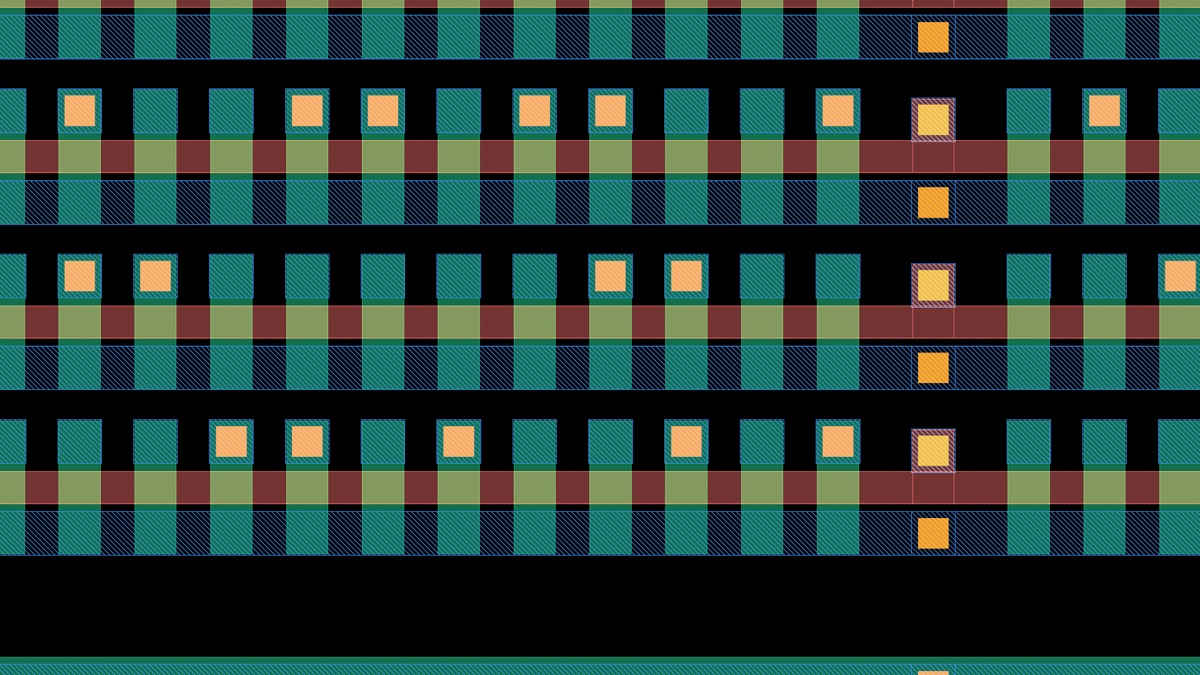
\includegraphics[width=0.49\textwidth]{figures/layout-weight-cells.jpg}\hfill
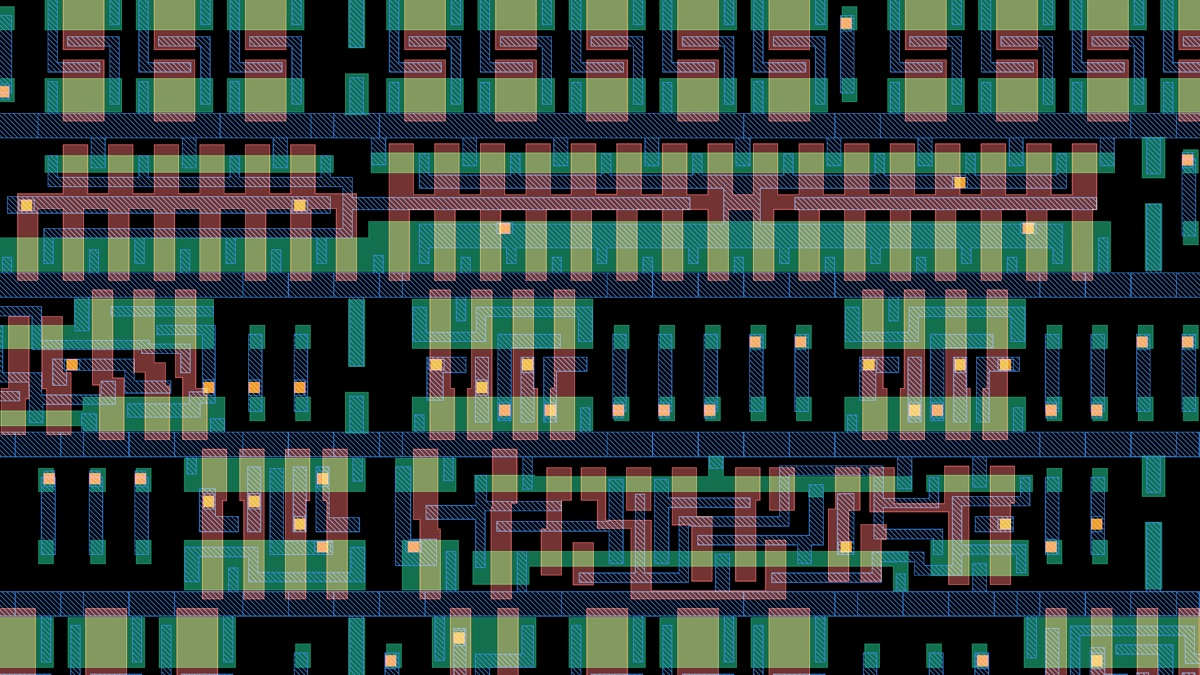
\includegraphics[width=0.49\textwidth]{figures/layout-engine-cells.jpg}
\caption{Layout close-ups rendered from the GDS (Via1 amber, Metal1 blue, poly and diffusion beneath; fill hidden). \emph{Left:} \SI{10.4}{\micro m}-wide window of weight bank \texttt{W13\_ENC0\_B00}. Each 4-bit index uses four mask-programmed access transistors; the irregular Via1 pattern over the regular cell grid sets the stored bits. \emph{Right:} \SI{29.5}{\micro m}-wide window of the routed $1280\times320$ engine (fix~2): standard cells of the select-and-accumulate datapath. Zoom sequences from full die to cells are in the release package (\cref{app:artifacts}).}
\label{fig:layout}
\end{figure*}

\paragraph{Power.}
Activity comes from a zero-delay gate-level simulation of one real-speech projection on the synthesized netlist. All 320 FP32 outputs of that run are bit-exact. Annotated against the final routed database and extracted parasitics, estimated engine power is \SI{0.188}{W} at TT and \SI{150}{ns}: \SI{142}{mW} combinational, \SI{24}{mW} sequential and \SI{21.5}{mW} in the clock tree. That is \SI{117}{\micro\joule} per projection, or \SI{287}{pJ} per MAC.

These are tool estimates, not silicon measurements. There is no matched multiplier-based GF180 baseline, so the result does not establish an energy advantage over conventional MAC hardware. Cross-node operation-energy comparisons~\cite{horowitz2014energy} require matched precision, workload, memory, voltage and physical scope. The flattened power report separates combinational, sequential and clock power, but does not isolate the integer core from FP32 affine logic. A per-module breakdown remains open.

The pre-route estimate for the same engine was \SI{162}{pJ}/MAC; that figure had no clock tree and only placement parasitics. Pin annotation was 67.5\%; the remaining pins are cells inserted after synthesis, which the analyser assigns default activity. The trend across iterations (241$\to$256$\to$287\,pJ/MAC) therefore mixes real design change with falling annotation coverage.

\subsection{Whole-recognizer synthesizability}
Synthesizing the complete recognizer flat failed for both silicon and FPGA. Synthesis tools stalled for hours in memory and flip-flop optimisation passes, and the FPGA run crashed. We therefore black-boxed the weight ROMs and synthesized the remaining 30,545 elaborated modules as 4,457 distinct units, each under a 6\,GB memory limit. All 4,457 units pass for a generic library, for GF180, and for the Lattice ECP5 FPGA family.

These separately synthesized units give an upper-bound-style estimate without cross-boundary optimization or weight-ROM interiors, not a placed or fully integrated netlist. The composed GF180 logic estimate is \SI{1198}{mm^2} (\SI{11.98}{cm^2}) (48.4\,M cells, 8.07\,M flip-flops), because all \num{8169778} bits of mutable state (buffers, caches, normalisation state) become flip-flops when no SRAM macros are inferred. That is $19\times$ the \SI{63}{mm^2} logic budget of our floorplan. The ECP5 mapping needs 30.4\,M LUT4s, 1.34\,M flip-flops, 1,247 DSP blocks and 118 BRAMs, far beyond any device in the family. The seven converted storage services alone (\num{139980800} bits) also exceed on-FPGA memory by more than an order of magnitude.

\subsection{Toward a full chip}
Several physical parts of the full chip exist but are not integrated:
\begin{itemize}
\item \textbf{Weight arrays.} All 98 weight matrices (\num{31457280} selections) are laid out as 81 pitch-matched index banks totalling \SI{174.7}{mm^2}. Every bank passes the selected DRC rules and GDS bit-pattern readback; density and antenna are outside that bank check. Full LVS passes on six representative banks, not all 81. A single bank measures \SI{5.54}{\micro m^2} per selection for its bank-local layout.
\item \textbf{Bank drivers.} Four driver/control shapes pass their selected DRC and LVS checks and meet \SI{150}{ns} across nine corners. Complete capture and array-periphery qualification remains open.
\item \textbf{Logic macros.} Six leaves meet the workstream's local READY criteria, which defer density to chip fill. Supplemental density checks still fail (five or seven markers per leaf); this is not complete block signoff.
\item \textbf{Two-die top level.} Two $25\times29$\,mm outlines contain 48 real banks, four logic leaves and 119 stubs, with bank drivers pending. Only 14 scalar nets are source-matched; 1,368 are synthetic test nets. Top wiring passes its routing checks, but minimum density remains unmet and assumed-load IR fails (VDD/VSS: A 0.869/0.866\,V, B 1.44/1.35\,V). Full-chip DRC completion, LVS and STA remain open; no complete neural datapath is demonstrated.
\end{itemize}
\Cref{sec:limitations} discusses what remains.
